\documentclass{ltjsarticle}
\usepackage{docmute} 
\usepackage{myStyle} 


\begin{document}
\chapter{帰無仮説検定の注意点}
\label{chapter19}
この報告の仕方について，次のセクションで少し解説しておきましょう。

\section{結果の報告の仕方}
帰無仮説検定を行った後の，報告の仕方について説明しておきましょう。

帰無仮説と対立仮説のモデル対決なので，結果は軍配をはっきり示す必要があります。帰無仮説が勝ったのか，対立仮説が勝ったのかを明記するのです。ちなみに仮説が勝った，というのを\keyterm{採択}{さいたく}{accept}，負けたというのを\keyterm{棄却}{ききゃく}{reject}と言うのでした。ですから「帰無仮説を棄却して対立仮説を採択」，あるいは「帰無仮説が棄却できずに採択，対立仮説を棄却」のどちらかになります。

また，結果の判定ですから，判定に使った数字＝検定統計量も報告する必要があります。相関係数の検定の例では，$t$統計量が使われましたので，これを報告します。また，$t$統計量は$t$分布に従い，これはサンプルサイズに依存する自由度によって調整されるものですから，自由度も報告する必要があります。今回の例ですと，次のように報告しましょう。
\begin{quote}
標本から得られた標本相関係数$r=0.50$について仮説検定を行ったところ，$t(18)=2.450,p=0.012$で統計的に有意であった。
\end{quote}
書き方のポイントとしては，統計量を書くこと，そしてその時の統計量はイタリック(斜体)であること\footnote{字体を整えるのは，心理学だけでなく論文の書き方として一般的です。統計量や本のタイトルなどはイタリックであることが決まっています。誰が決めているかって? America Psychological AssociationのPublication Manualにそう定められていますし，日本の心理学会も基本的にこれに準じた出版作法を定めているのです。}，その統計量の実現値が得られる確率($p$値)を記載すること，です。

$p$値は上の例のように確率そのものを描くのが基本ですが，昔は判定基準を使って$p<0.05$とか$p<0.01$と書いていました。これは手計算で検定をしていた頃の名残で，統計環境Rなどがなかったものですから確率計算が直接できませんでした。ではどうしていたか，というと代表的な確率分布の数字が載っている数表\footnote{昔は確率分布の数字の一覧が載っている本がありました。確率のテキストには付録として，数表の一部が載っているものもあります。}を使ってチェックするしかなかったので，細かい数字まで計算できなかったのです\footnote{例えばt分布は自由度によって変わりますが，自由度$1,2,3\cdots$と1つずつ書いてあったのでは，付録のページ数がいくつあっても足りません。そこで$1,2,3...10,15,30,50$のように，後半の方は「だいたいこれぐらい」という大雑把な幅でしか載っていませんでした。こんな時，じゃあ自由度18ならどうしたらいいんだ，と思うかもしれませんが，その時は手元のデータに最も近く，より厳しい自由度15のところを見て代替する，というやりかたでした。ですから具体的な$p$値は書けなかったのです。}。今ではそういう問題がないので，そのまま$p$値を書きましょう。

\section{統計的に有意，とは}
\label{sec::18_04}
さてここまで，(ひとつの)平均値の検定や，相関係数の検定を行なってきました。
想定された平均値と大きく違っている/いない，とか，母集団での相関関係がある/ない，という事例でしたが，最終的には帰無仮説を棄却する/採択する，という話になるのでした。

この時，帰無仮説が棄却できると「統計的に有意statistically significant」ということがあります。統計的に意味がある，というわけです。ただし気をつけて欲しいのは，統計的に有意とはどういうことか，です。
相関係数の検定の時のことを思い出しましょう。帰無仮説は$\rho=0$というものでした。これが棄却されたので，「統計的に有意な相関係数だ」と結論づけたわけですが，より正しくは「母相関が0であるとはいえない」ということですよね。関係がないとは言えない$\to$関係がある，というこの$\to$の部分は，厳密に言えば少し飛躍があることになります\footnote{「あなたのことが嫌いではない」といわれても好きだとは言ってないわけで。}。

この帰無仮説検定を考えた人は，R.A.フィッシャーという人なのですが，この人は帰無仮説が棄却されたら「なにかおかしなことが現実に起こっているのだから，実験手続きを見直したほうがいい」というチェックのために使うことが想定していました。これをE.ピアソンとJ.ネイマンという人が「帰無仮説の棄却＝対立仮説の採択，とすれば良い」という判断基準と合わせて使う方法への応用したのです。心理学ではその流れを受けて帰無仮説検定を利用してきました。そういう意味で，本来の創始者の意図とは違った，より実践的な意味のある(言い換えれば実用上の責任を負わなければならない)使い方をしているのです。

また既に述べたように，実際の相関係数の大きさや，平均値の差についての情報がかき消された表現になっていることにも注意が必要です。例えば，標本を多く取れば標本相関係数が$r=0.1$でも帰無仮説を棄却して統計的に有意である，ということができます\footnote{実際に，サンプルサイズが271人を超えると，5\%水準で有意になります。
}。
これで「統計的に有意だ！無相関とは言えない！」と言っても，標本相関係数が0.1なのですから，「(相関)関係がある」という結論で議論するとおかしなことになるわけです。

ところが実際，このような表面上の使われ方に引っ張られてしまうことはよくあります。特に研究をしていると，努力したのに関係がなかった，と言いたくないという気持ちが働いてしまいます。そこで，有意になったんだから意味はあるよね，と考えて無理やり二変数間の関係を考察してしまう，ということになってしまいます。これではせっかくデータを取ったのに，正しく考えられたことになりません。

また一般に，サンプルサイズが大きいと帰無仮説は棄却しやすくなります。図\ref{fig::18_02}には，横軸にサンプルサイズ，縦軸に$p$値をとり，標本相関係数が$r=0.5,0.3,0.1$のときにどうなるかをプロットしました。5\%を有意水準(点線)としていますが，サンプルサイズが大きくなるにつれて$p$値は小さくなって行きます。

\begin{figure}[ht]
    \centering
    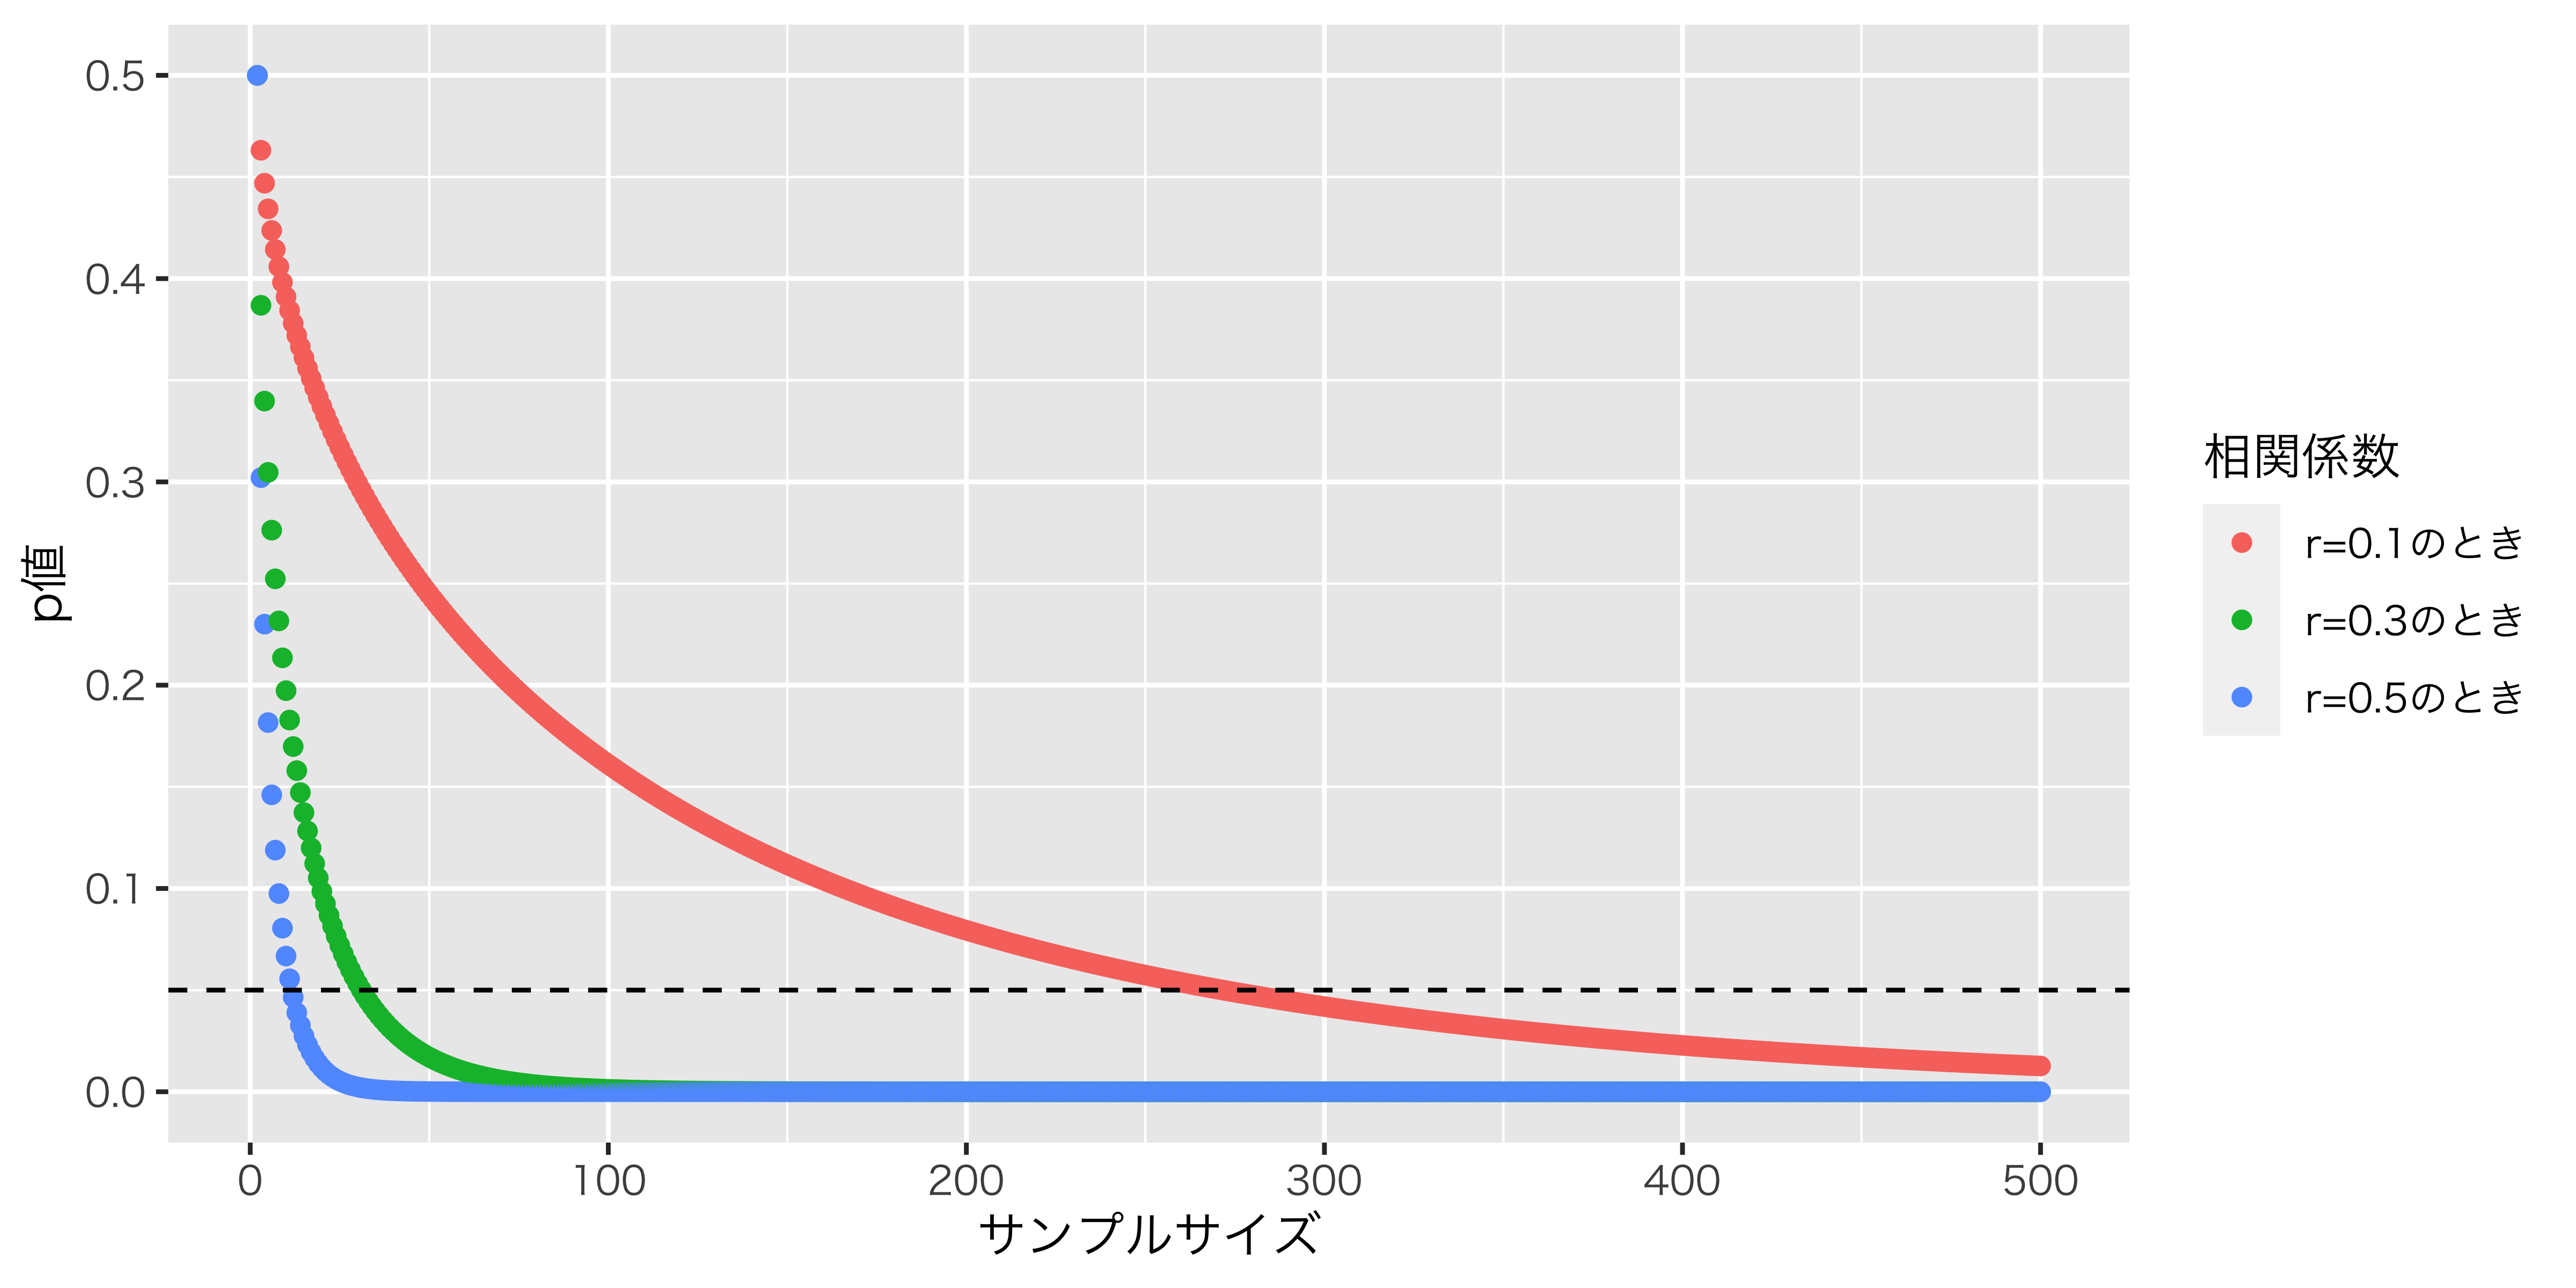
\includegraphics[keepaspectratio,width=12cm]{images/text18/Rplot18_02.png}
    \caption{サンプルサイズと$p$値の関係}
    \label{fig::18_02}
\end{figure}

この下がり方はどこからスタートするかにかかわらず同じ形ですから，判定はサンプルサイズが増えさえすればいずれ有意になるのです。これがまた，研究の実践ではおかしな風潮を呼んでしまいます。つまり，\underline{有意にしたければ}サンプルサイズをたくさん取る＝頑張れば良いのです。

科学的に正しいかどうかを考えるべきシーンで，「頑張れば有意になる」といった``努力''に依存するのはおかしいことだと思いませんか。頑張った$\to$有意になった$\to$著者の主張が正しい，というのは，論理的ではありません。結果を自分の都合の良いように変えることは，正しい努力ではないはずです。

帰無仮説検定は，標本から母集団のことを「判定」できる優れた技術ですが，表現とその解釈に気をつけないと，科学を間違った方向に導きかねないことに注意が必要です\footnote{残念ながら，これまでの心理学の歴史の中でもこのような間違った努力がなされてきた事実があります。これらはQRPs(Questionable Research Practices：QRPs＝問題のある研究実践)と言われています。}。

\section{検定における2種類の間違い}
\label{sec::18_05}
最後に，確率を伴った判定の仕方について考えておきましょう。
先ほどから，確率を$p$値と呼んで説明してきましたが，さて，この$p$値は何を表している数字でしょうか？ 

\begin{itemize}
    \item 帰無仮説の生じる確率
    \item 帰無仮説の正しさを表している数字
    \item 有意差の大きさを表している数字
    \item 検定の強さを表している数字
\end{itemize}

正解は，上のどれでもない，です。意地の悪い選択肢でごめん。
上の2つの選択肢，「帰無仮説の生じる確率」「帰無仮説のただしさを表している数字」はよくある引っ掛けなのですが，仮説検定は「帰無仮説の下で・・・」という前提から始まります。無相関検定のときに，母相関が0の世界から標本をピックアップする例をお話ししましたね。母相関の世界を前提として・・・という話なので，帰無仮説の生じる確率は100\%，帰無仮説の正しさも100\%です(だって仮定したんだから！)。

有意の程度の大きさを表す数字でもありません。確かに差が大きいとか，帰無仮説の世界から大きく離れているというようなことがあれば，検定統計量の実現値は大きくなり，$p$値は小さくなります。が，$p$値が示しているのは(帰無仮説の下での)検定統計量の出現確率であり，いわば帰無仮説という仮想空間の中での数字であって，現実の統計量について何か示す数字ではないのです。

検定の強さを表す数字，でもありません。$p$値が小さくなればなるほど，確かにレア度は増しているのですが，それは帰無仮説という仮想空間の中でのレア度であって，帰無仮説が対立仮説をどれほど打ち負かしたか，という情報を持っているわけではありません。ですから，$p$値が小さければ小さいほどすごい，などと思ってしまうと本質を見誤ります。

では検定の正しさや間違いについて，どのように考えれば良いのでしょうか。実はこれも，確率的表現の難しさがあるのです。
帰無仮説検定最後のステップでは「最初に定めた仮説が間違っているか正しいかを判断する」というのがありました。この判断の間違い方にも，2種類あるのです。つまり，「帰無仮説が正しいのに棄却してしまう」という間違い方と，「帰無仮説が正しくないのに採択してしまう」という間違い方です。

\begin{figure}[ht]
    \centering
    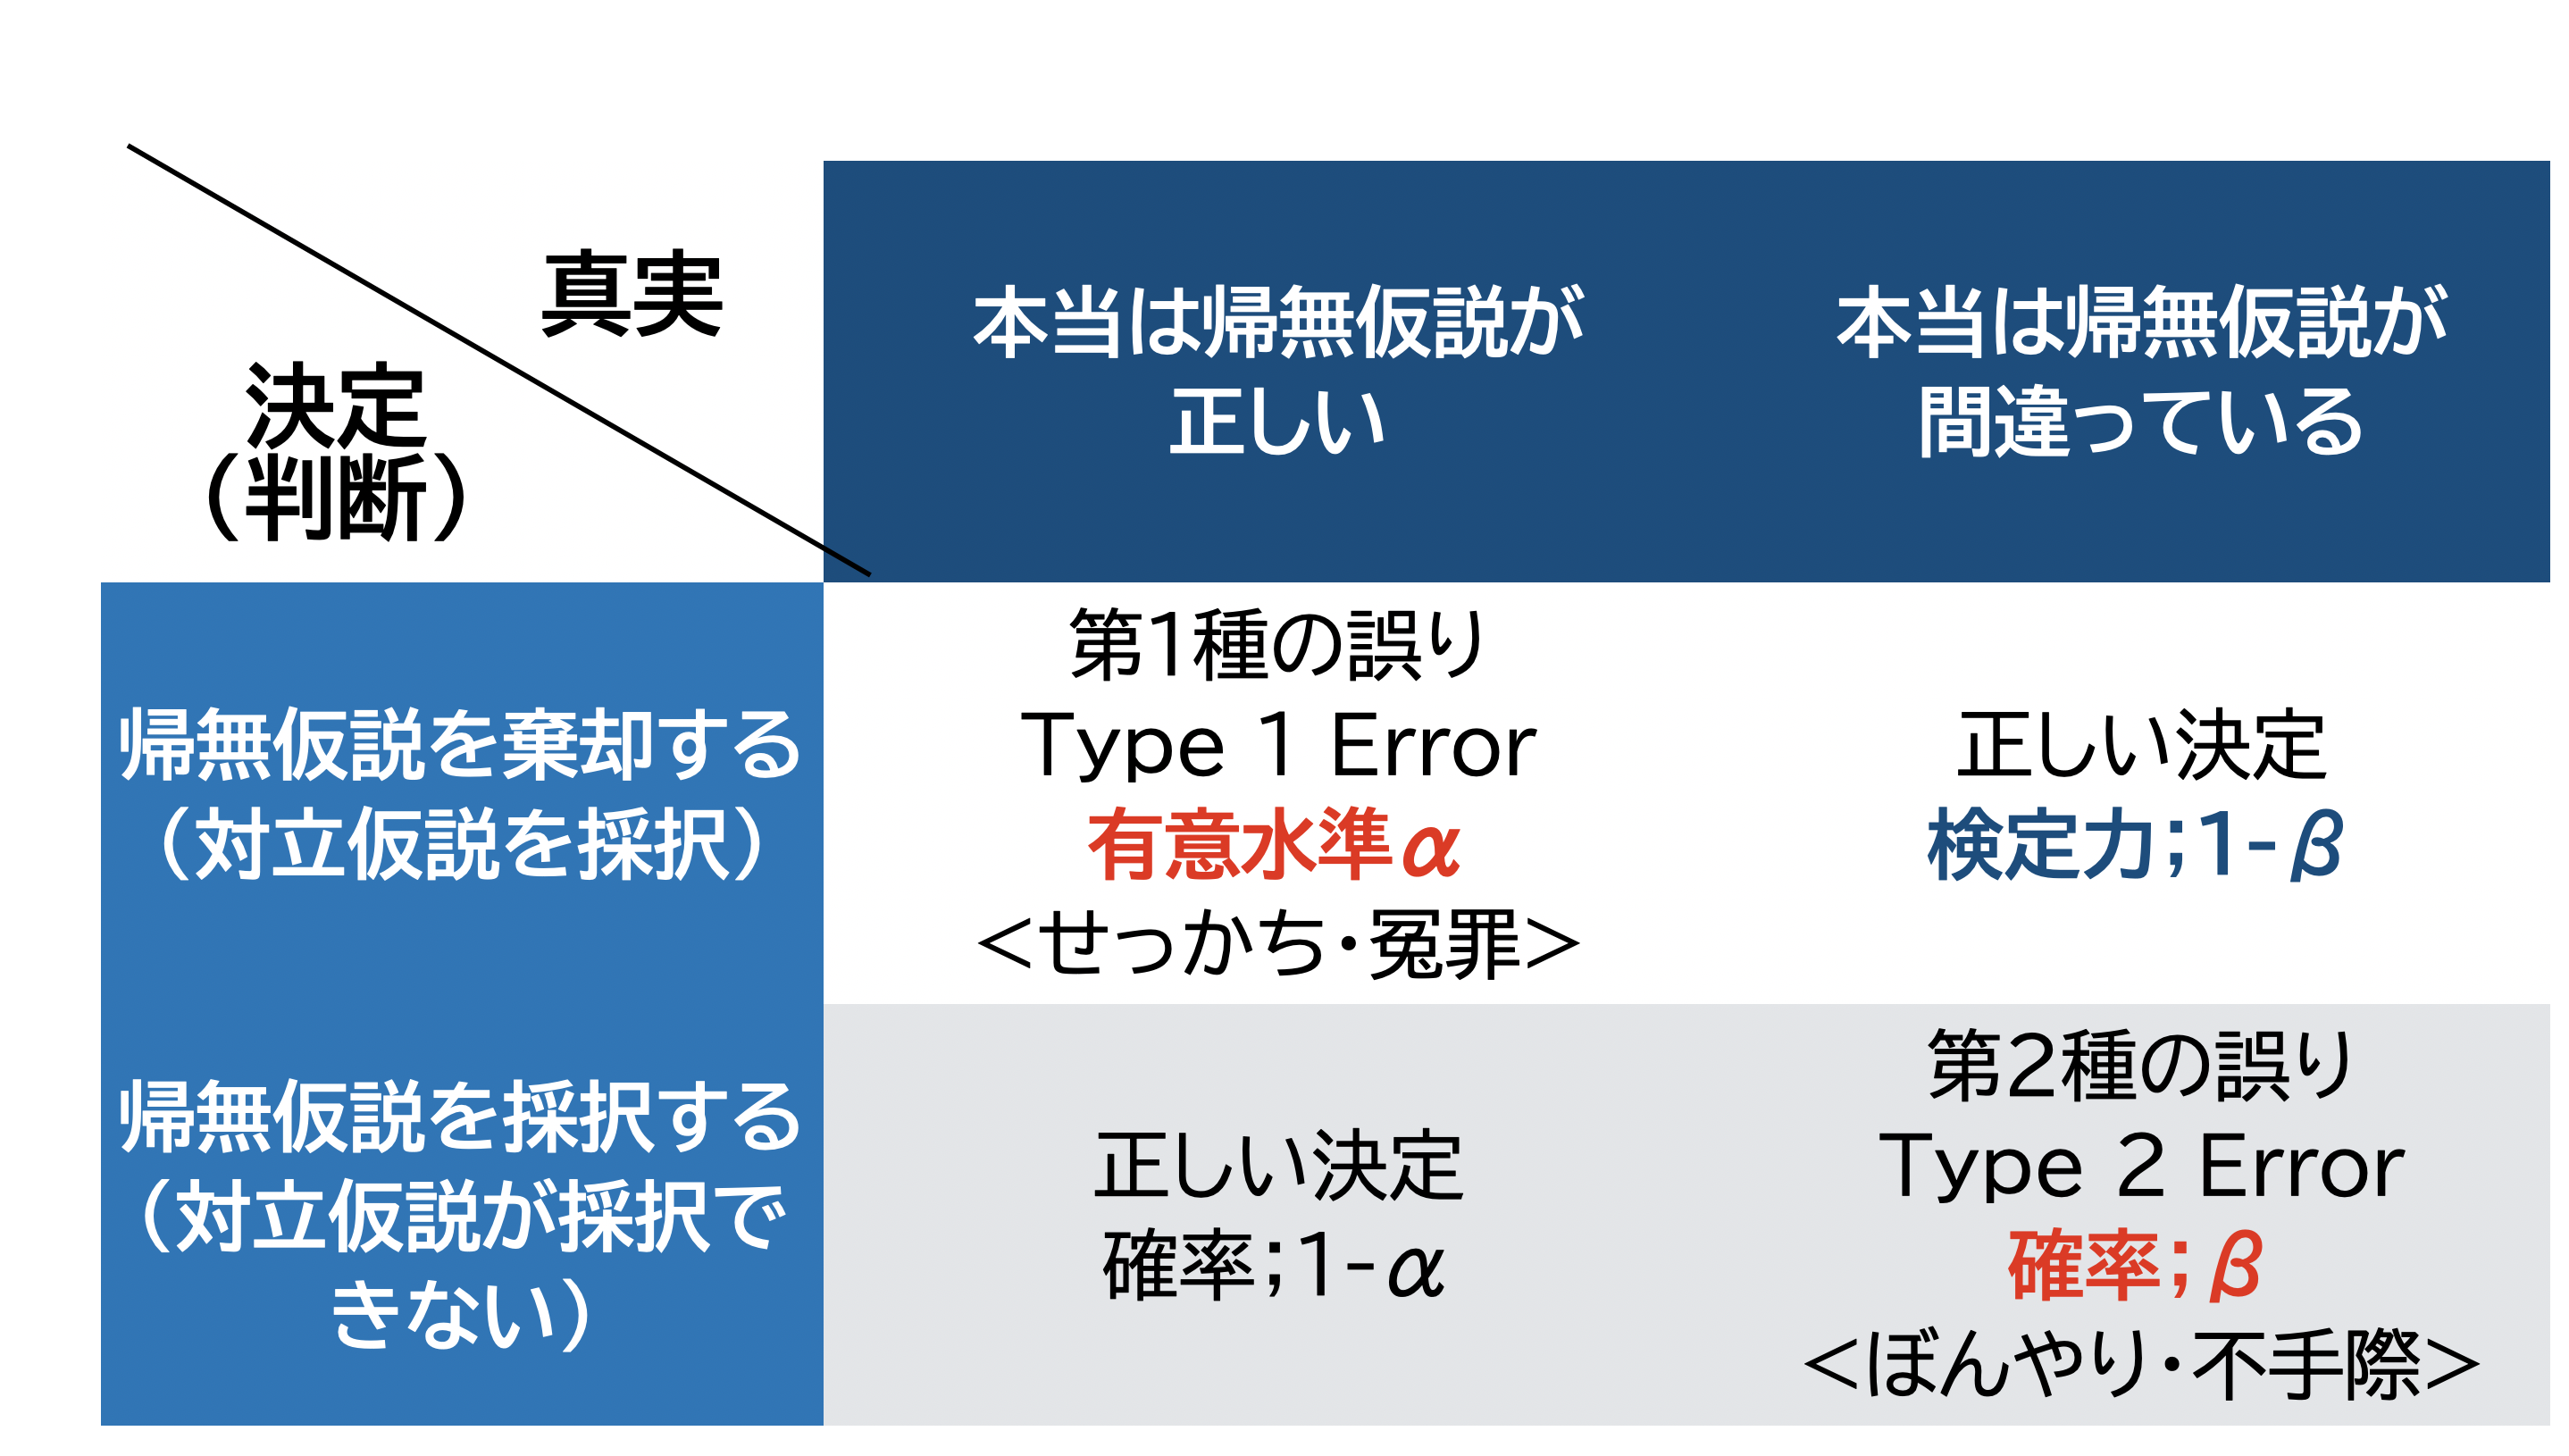
\includegraphics[keepaspectratio,width=12cm]{images/text18/slide18_01.png}
    \caption{二種類の間違い方}
    \label{fig::18_03}
\end{figure}
図\ref{fig::18_03}に，間違い方の組み合わせを書いてみました。帰無仮説が正しいときに帰無仮説を採択する，帰無仮説が正しくないので帰無仮説を棄却する。これができれば正しい決定ですが，「帰無仮説が正しいのに帰無仮説を棄却する」のも「帰無仮説が正しくないのに帰無仮説を採択する」のも間違いです。
帰無仮説は差がないとか効果がない，といったNullな結論です。ここでは仮に，開発された新薬に治療効果があるかどうかを考えている，というシーンを想像してみてください。帰無仮説はこの新薬に効果がないときです。ロクな効果がないときに，帰無仮説を棄却する＝対立仮説を採択する＝効果があると言ってしまうのは，怖いことですね(患者さんに副作用など悪影響があるかも！)。このような功を焦って誤った判断をしてしまう危険な間違いを，\keyterm{第一種の誤り}{だいいっしゅのあやまり}{Type I Error}とよび，その確率を$\alpha$で表します。実は，5\%水準で判断するというのは，この$\alpha$の確率を0.05にしたことになります。慣例では$\alpha=0.05$となっていますが，別に1\%でも10\%でも，自由に決定して構いません。どの程度の水準にするかは，この間違いを犯した時の重要さを参照しながら決めるべきことです。

一方，効果があるのに（帰無仮説が間違ってるのに)，帰無仮説を採択するのは，せっかくの効果を見抜けなかった残念なケースです。これも困った結果ではありますが，少なくとも患者に迷惑がかかるようなことはありませんよね。なので，こちらについてはひとまず間違っても実際的な問題は生じないでしょう。こちらのケースは\keyterm{第二種の誤り}{だいにしゅのあやまり}{Type II Error}と呼び，確率は$\beta$で表すのが一般的です。ただ，この$\beta$は帰無仮説が間違っている，つまりNull「でない」状態が，どう「である」のかわからないので，大きさを見積もることはできません。せめて，効果があるときはちゃんとあるって知りたいよね，と思いを馳せるだけです。この図\ref{fig::18_03}にある表は，列ごとに世界線が分かれていますから，右列の「帰無仮説が間違っている世界」で「帰無仮説を棄却してしまう確率」が$\beta$であれば，ちゃんと効果を見つけ出せる確率は$1-\beta$です。この$1-\beta$を\keyterm{検定力}{けんていりょく}{power}といい，検定力のある分析ができているかどうかをちゃんとチェックしておくのは，研究の手続き上重要なことです。

検定力のチェックは，分析が終わった後に事後的にすることもできますし，事前にすることもできます。事前に，というのは，みたい効果がどの程度あるのかを考え，その効果をきちんと検出するにはサンプルサイズをどれぐらいにすれば良いのかを考えること，でもあります。このサンプルサイズを考えることを，\keyterm{例数設計}{れいすうせっけい}{sample size design}といいます。

帰無仮説検定において，例数設計はとても大事なことです。既に述べたように，サンプルサイズが大きくなると有意だという判断はしやすくなります。これは$p$値で判断する以上仕方のないことですが，だからと言ってそれを逆手にとって，事実よりも主張をするためにサンプルをたくさんとるのは，帰無仮説検定のハッキングのようなものです。ですので，検定をするときはまず「どの程度の効果が見込まれ，これを検証するためには何人ぐらいのサンプルをとらなければならない」と宣言してから，検定して判断するという手続きが必要です。この宣言をせずに検定をすると，「有意にするためにサンプルサイズを変えたのではないか」と批判されてしまうかもしれません。

学部の授業や卒論で行う実験で，例数設計をしたりサンプルサイズの宣言をするようなことはないかもしれませんが，学術業界では事前に学会にこの宣言を伝えてから研究に取り掛かる，事前登録制pre-registrationが導入されはじめています。
\end{document}
